\scanpage{13}
% L1
\deleted{\uline{Lemme}}\inserted{\uline{Prop}} Soit $G$ \inserted{$=\underline{\mathrm{Aut}}(Y)$ ($Y$ droite projective)} forme de $GP(1)$ sur corps $k$ \inserted{alg. clos}, $\tau_0,\tau_1,\tau_2\in G(k)$
% L2
tels que $\tau_0^2=\tau_1^2=\tau_2^2=(\tau_0\tau_2)^2=1$. Conditions équivalentes

% L3
A) $\exists$ \deleted{diviseur} diviseur de degré $2$ sur $Y$ \deleted{tel que}\inserted{stable} par les $\tau_i$

% L4
\leavevmode\llap{\smash{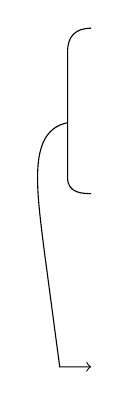
\begin{tikzpicture}[baseline=0pt,x=1mm,y=1mm]
\draw (0,2) .. controls (-2,2) and (-3,1) .. (-3,-1) -- (-3,-17) .. controls (-3,-19) and (-1,-19) .. (0,-19);
\draw[->] (-3,-10) .. controls (-8,-11) and (-7,-18) .. (-6,-26) -- (-4,-41) -- (0,-41);
\end{tikzpicture}}\hspace{1mm}}B) On peut trouver un sous groupe \deleted{alg\unsure{éb}} $H$ de $G$ qui est
% L5
soit \quad a) un $N(T)$, $T$ tore maximal
% L6
\hphantom{soit}\quad b) un $B$, sg groupe de Borel
% L7
tel que les $\tau_i\in H$

% L8
A') Les \deleted{repr. project.} prolongem\unsure{ts} \deleted{projectifs} \inserted{$\tau'_i$ au plan projectif enveloppe $C$} \deleted{\unsure{$\varphi$}} $(i=0,1,2)$
% L9
des $\tau_i$ laissent une droite invariante ($\Leftrightarrow$ si
% L10
car. est $\ne2$ : laissent un pt invariant)

% L11-13
\deleted{C) L'image de \deleted{\unsure{la|des}} $G_2^+$ dans $G(k)$ [i.e. le gpe engendré par $\rho_0=\tau_0\tau_1$ et $\rho_1=\tau_1\tau_2$, ou par $\rho_0$ et $\sigma=\tau_0\tau_{2}=\rho_0\rho_1$] est commutatif}
% L11a
\margin{C''') $\varphi$ se factorise par un groupe $\Gamma'$ ext. \deleted{centrale d'un}\inserted{d'un gpe comm.} \deleted{ce gpe :} par un groupe \uline{cyclique}}
% L13a
\margin{C') $\varphi:G_2\unsure{\mathbin{-}|\to}G(k)$ se factorise à travers un $\mathbb D_\infty\times\mathbb Z_{/2}$}

% L14
\deleted{\unsure{B|C}}\uline{C}) Deux parmi les trois couples $(\tau_0,\tau_1)$ $(\tau_1,\tau_2)$
% L15
$(\rho_0,\rho_1)$ commutent, i.e. ou $\rho_0^2=1$ ou $\rho_1^2=1$ ou $\rho_0\rho_1=\rho_1\rho_0$

% L16
\uline{D}) Le \deleted{\unsure{noyau dans un des op.}}\inserted{ss-groupe de $G(k)$} engendré par les $\tau_i$ est
% L17
isom à un $\mathbb D_n$ ($n\geq1\unsure{\}},$ y c. infini) ou $\mathbb D_{\unsure{n|m|\infty}}\times\mathbb Z_{/2}$ ($n$ pair)
% margin note written sideways
% L17a
\margin{\uline{NB} dans (D), si car $k\ne2$, on peut remplacer les $\mathbb D_n\times\mathbb Z_{/2}$ par $\mathbb D_\infty\times\mathbb Z_{/2}$}

% L18
$A\Leftrightarrow A'$ $\deleted{\Leftrightarrow}$ : traduction via dictionnaire entre $Y$ et $C$ (div. de degré
% L19
$2$ sur $Y\longleftrightarrow\text{droites de }C$)

% L20
$A\Longleftrightarrow B$ car les stabilisateurs des div de degré $2$ sur $Y$
% L21
sont les ss-gpes explicités dans B

% L22
On utilisera que les groupes $H(k)$ sont des produits
% L23
$1/2$-directs $\unsure{\gamma|\mathcal T}.U$, $U$ comm, $\gamma$ \deleted{\unsure{d'un gpe}}\inserted{comm.},
% L24
$ {}_2\gamma$ d'ordre $1$ ou $2$, \unsure{$1/2$ entier|$1/2$ enfin} $ {}_2U$ dans le centre de \deleted{\unsure{de $H$}},
% L25
\deleted{\unsure{et pour voir que}}\inserted{$i_{\varepsilon}$ est l'identité sur $ {}_2U$}. $({}_2\gamma).U$ \unsure{lire|i.e.} $ {}_2\gamma=\{1\}$ ou $ {}_2\gamma=(1,\varepsilon)$, avec \unsure{$\varepsilon\ \mathrm{int}\ \varepsilon\mid H$}.

% L26
$B\Longrightarrow C$ \qquad En effet, \deleted{comme alors} les images des $\tau_i$ dans
% L27
$\gamma$ étant dans $ {}_2\gamma$ \deleted{sont égales} si $ {}_2\gamma=\{1\}$, \deleted{\unsure{que}}\inserted{cas $H=B$},
% L28
en car. $2$) alors l'image $\Gamma'$ de $\Gamma$ dans $G(\unsure{s|k|S})$
% L29
est $\subset H(k)$ donc est comm, on a C.
% L30
Sinon, soit $\gamma=\{1,\varepsilon\}$. Si \deleted{$(\tau_0,\tau_1)$ et $(\tau_1,\tau_0)$}
% L31-32
\deleted{$\tau_0$ et $\tau_1$, $\tau_2$ \unsure{ts} égaux à $1$, c'est comme dessus. Si $\tau_1\,\tau_0$ ne commutent pas, on voit que \unsure{$\tau_2$}}
% L33
on avait $\tau_i\in H(k)$, comme $\tau_i^2=1$, on
% archive sheet number: 12
